The measuring module is in charge of calculating all the selected writing style metrics. In order to measure these features, it receives from the \textit{Analyser} class a corrected message with the following structure (which matches with the corrected messages' structure):

\begin{python}
	{
		'id' : string,
		'threadId' : string,
		'to' : [ string ],
		'cc' : [ string ],
		'bcc' : [ string ],
		'sender' : string,
		'depth' : int,               # How many messages precede it
		'date' : long,               # Epoch ms
		'subject' : string,
		'bodyBase64Plain' : string,
		'plainEncoding' : string,
		'charLength' : int,
		'corrections' : [
		{
			'text': str,
			'is_punct': bool,
			'is_right_punct': bool,
			'is_left_punct': bool,
			'like_url': bool,
			'like_email': bool,
			'lemma_': str,
			'is_stop': bool,
			'pos_': str,
			'is_bracket': bool,
			'position': int
		}
		]
	}
\end{python}

\begin{figure}[p]
	\centering%
	\centerline{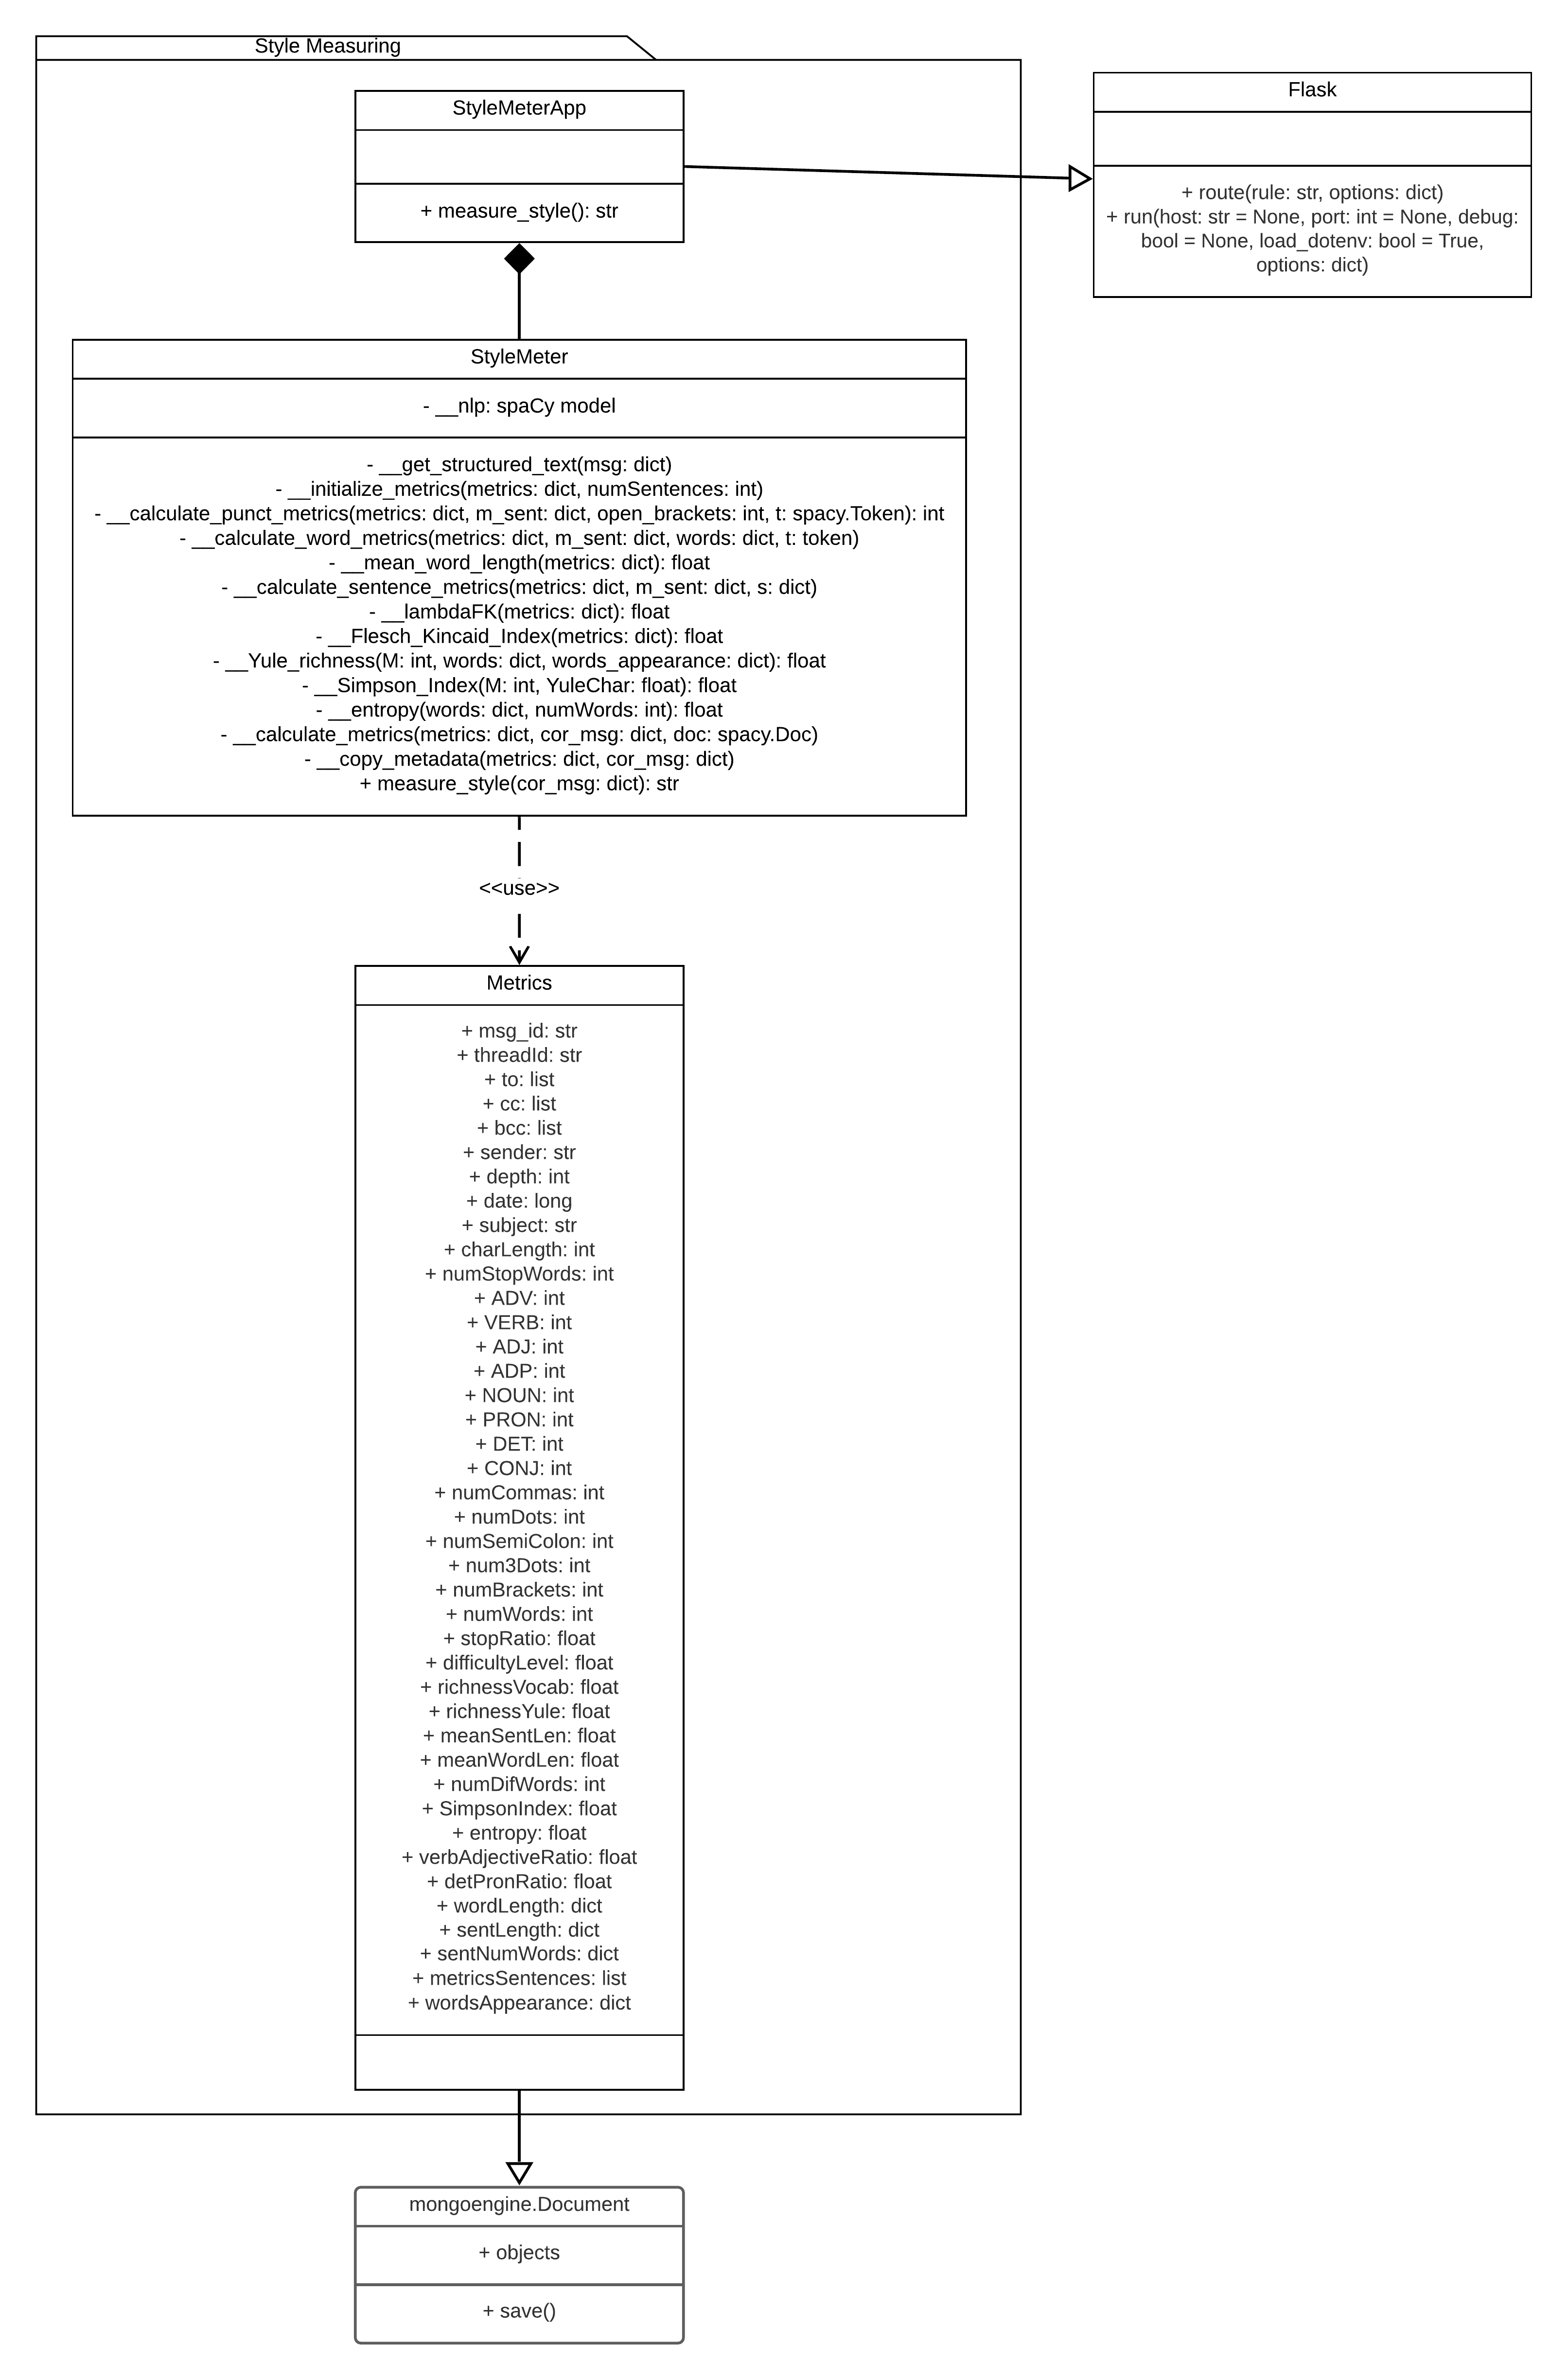
\includegraphics[height=0.8\paperheight]{Imagenes/Bitmap/Analyser/metUML.png}}%
	\caption{UML class diagram of the measuring module}%
	\label{fig:umlmet}
\end{figure}

As we can see in Figure \ref{fig:umlmet}, the style measuring package has three different classes with a class diagram similar to that of the preprocess package. These three classes are: \textit{StyleMeterApp}, \textit{StyleMeter} and \textit{Metrics}.

As with the two previous modules, this package implements a Flask web service which can be used through a POST HTTP request with the message as a \textit{json} in it. Having done so, the \textit{measure\_style} method of the \textit{StyleMeterApp} class is invoked and sends the given message structure to the \textit{StyleMeter} class by calling its only public method: \textit{measure\_style}.

The main class of this UML package is the \textit{StyleMeter} class. It is in charge of calculating the style features. For this reason, it has different methods which implement the distinct style markers that it has to evaluate.

As the reader is able to deduce after presenting the previous sections, the \textit{Metrics} class stores in the database the results of measuring each message. The \textit{StyleMeter} class uses it once it has calculated all the style characteristics.

We have used 31 lexical-syntactic features (due to previous studies, such as that conducted by \cite{homem2011authorship}, yield encouraging results with lexical-syntactic features), following the classification of \cite{abbasi2008writeprints} (which categorised stylistic features as lexical, syntactic, structural, content-specific and idiosyncratic style markers), and we will now divide them into four categories in which we have grouped them according to their usefulness in terms of what type of conclusions we can infer from each of them. These categories are: part of speech features (see Section \ref{ssect:posf}), punctuation features (see Section \ref{ssect:punctf}), vocabulary features (see Section \ref{ssect:vocabf}) and structural features (see Section \ref{ssect:strucf}). We must not confuse this latter category (which belongs to the lexical features of the classification given by \cite{abbasi2008writeprints}) with the structural metrics explained by \cite{abbasi2008writeprints}. Some of the popular metrics which are not used in this work, belong to the structural, content-specific and idiosyncratic style markers of \cite{abbasi2008writeprints}, but there are others which belong to the same categories as the explained metrics (lexical and syntactic).

The choice of the metrics presented below, some essentially simple, has been directed by the objective of finding easily explainable characteristics that set the parameters of the style of writing according to the recipient of the e-mail. In addition to it, we are interested in being able to draw conclusions from the results obtained with the metrics and use them to develop, in future projects, systems of natural language generation of e-mails that take into account this factor. Indeed, the last part of this work is a personalised writing model based on the recipient which takes in advantage the conclusions that we present in this work. For this reason, some excessively complex metrics, although popular in stylometry (such as n-grams), have been avoided and an attempt has been made to prioritize the explainability of the chosen features.

Finally, we relate the explained style markers with their implementation (see Section \ref{ssect:relmet}) in the \textit{Metrics} class.

\subsection{Part of Speech metrics}\label{ssect:posf}

We will call our part of speech metrics as the syntactic features which have to do with the part of speech of each word of the e-mails. Following the suggestion of \cite{holmes1985analysis}, we count the number of nouns, verbs, adjectives, adverbs, pronouns, determinants, conjunctions and prepositions of each text. By calculating this, significant stylistic traits may be found, because as \cite{somers1966statistical} claims: ``A more cultivated intellectual habit of thinking can increase the number of substantives used, while a more dynamic empathy and attitude can be habitually expressed by means of an increased number of verbs. It is also possible to detect a number of idiosyncrasies in the use of prepositions, subordinations, conjunctions and articles''.

In addition to this metrics, we calculate the verb-adjective ratio and the determinant-pronouns ratio, proposed by \cite{antosch1969diagnosis} and \cite{brainerd1974weighting}, respectively.

\subsection{Punctuation metrics}\label{ssect:punctf}

In order to extract conclusions from this syntactic metrics, and following the example of \cite{calix2008stylometry}, we calculate the amount of commas, periods, semi-colons, ellipsis and pair of brackets. With these features we can reach conclusions such as the structural complexity of a message (since, for example, juxtaposition structures appear in the presence of some of these scores), the division into sentences of the message or the need for clarification of the text transmitted (for example, by analysing the amount of brackets).

\subsection{Vocabulary metrics}\label{ssect:vocabf}

In terms of the used vocabulary, we work with the ``bag of words'' metrics, in other words, we note how many times each different word is used in a message. Of course this is not the only metric that we can categorise as a vocabulary feature and from which we can extract conclusions about the vocabulary used. There are many others which try to set the parameters of, for instance, the difficult of the vocabulary or its richness. Furthermore, from the computing of the bag of words, we are able to easily obtain other style marker chosen which also belongs to this category of vocabulary features: the amount of different words in each text, proposed by \cite{ril2014determination} and by \cite{corney2001identifying}.

As for the difficulty level, it determines the level of education that someone needs to have if they are to understand the text. There are several indices available to calculate this level, such as the proposed by \cite{dale1948formula}, the Gunning Fog Index \citep{wiki:gunning} or the Flesch-Kincaid index \citep{dubay2004principles}, although the latter is the most commonly documented and cited. The expression which determines the Flesch-Kincaid index is the following:

$$
I_{FK} = 1.599\lambda-1.015\beta-31.517
$$

Where $\lambda$ is the mean of one-syllable words per 100 words, and $\beta$ is the mean sentence length measured by the number of words. However, as our spaCy's pretrained Spanish model (see Section \ref{sect:spacy}) is not able to divide words by syllables, we determine $\lambda$ as the mean of words with two or less characters per 100 words.

In respect of the richness of the vocabulary, we have chosen two different metrics. The first that we are going to explain is the one proposed by \cite{honore1979some}, which determines the richness of the vocabulary based on the total unrepeated words used in the text. The following formula defines it:

$$
R_H = \frac{100\log(M)}{M^2}
$$

Where $M$ is the number of different words in the text. However, as \cite{ril2014determination} claims, depending on the type of document being analysed, the calculation of $R_H$ has more or less validity (for instance, certain specialist articles, as their nature, requires constant repetition of words). As a consequence of this, another definition of richness of vocabulary is proposed by \cite{yule2014statistical}. This richness marker, that we use as our second richness of vocabulary style marker, is called Yule's characteristic and defined with the following expression:

$$
K = \frac{10^4\left(\sum_{i = 1}^\infty i^2V_i-M\right)}{M^2}
$$

Where $M$ is the number of different words in the text and $V_i$ is the number of words that appear i times in the document.

From Yule's Characteristic we are able to calculate the Simpson's Index (denoted as $D$), defined by \cite{simpson1949measurement}. This famous metric is understood as the measurement of diversity based on the change that the two members of an arbitrary chosen pair of word tokens will belong to the same type. To calculate $D$ it is necessary to divide the total number of identical pairs in the sample by the number of all possible pairs, that is to say, what the following expression defines:

$$
D = \frac{\sum_{i = 1}^\infty i(i-1)V_i}{M(M-1)}
$$

Where we are maintaining the Yule's Characteristic notation. However, as we have transmitted in advance, it is possible to calculate the Simpson's Index if we know the value of Yule's Characteristic. This relationship is defined by the following expression (and we use it in the implementation in order to speed the computing):

$$
10^{-4}K=D\left(1-\frac{1}{M}\right)
$$

Vocabulary distribution can also be measured by using a concept linguists have borrowed from thermodynamics and applied to communication theory: entropy (used by \cite{holmes1985analysis}). In literary text it is true that with an increase in internal structure, entropy decreases, and with an increase in disorder or randomness, the measure of entropy increases. The expression for the entropy of a system (vocabulary in this case) is:

$$
H = -\sum_{i=1}^{\infty} p_i\log(p_i)
$$

Where $p_i$ is the probability of appearance of the i-th lemma (found by dividing the number of occurrences of that lemma by the total number of words in the text). Due to the value will change according to how much text is analysed, the formula may be refined in order that works of different length may be compared. In this way, as it is proposed by \cite{holmes1985analysis}, the following expression determines absolute diversity for any length text as 100, while absolute uniformity remains zero:

$$
H=-100\sum_{i = 1}^{\infty}p_i\frac{\log(p_i)}{\log(M)}
$$

In addition to the words distribution features (which are the bag of words and the amount of different words), the level of difficulty, the richness of vocabulary (which is measured by the formula proposed by \cite{honore1979some} and the Yule's Characteristic), the diversity (represented by the Simpson's Index) and the internal structure of the vocabulary (which is measured by the entropy), we have defined other four style markers which also allow us to extract conclusions about some feature of the vocabulary of the message. The first of these is the most popular and old style marker: the mean word length. Researchers as \cite{ril2014determination} claim that it is ``directly connected with the richness of the author's vocabulary and measures his or her ability to use complex words'', due to it is considered that complex words are formed by three or more syllables that do not represent proper nouns, prefixes, suffixes or compound words. Thus, \cite{ril2014determination} propose an expression similar to the following one in order to calculate it:

$$
L_W = \frac{\sum_{i=1}^{\infty}i*C_i}{N}\cdot 100
$$

Where $C_i$ is the number of words with $i$ characters and $N$ is the number of words used. This formula is analogous to the expression proposed by \cite{ril2014determination}, except that with the one that we have presented the punctuation marks are removed from the numerator.

The second of these writing style metrics is the measurement of words length frequency distribution, that is to say, how many words with one character appear in the document, with two characters and so on up to the length of the longest word. Despite of being strongly influenced by the language, it is used by researchers as \cite{corney2001identifying} and \cite{kemp1976personal}, as \cite{allen1974methods} claims: ``Each writer, however, will have his own curve, so that although English (and German) texts in general peak at three letters, the writings of John Stuart Mill peak at two and those of Shakespeare peak at four''. Our interest will then focus on checking whether, in addition to depending on the author, this metric varies according to the recipient of the e-mail.

The rest of vocabulary features are related to the stop words present in the text. The simplest of those metrics is the style marker which consists of calculating the total number of stop words (denoted as $T_S$). On the other hand, as it is proposed by \cite{ril2014determination},  we will calculate the stop words ratio, which is defined with the following expression:

$$
S_W = \frac{T_S}{N}\cdot 100
$$

\subsection{Structural metrics}\label{ssect:strucf}

We will denote by structural metrics those features that we obtain directly from the construction of the analysed text. Some of these style markers are as simple as the total number of characters in the body of the e-mail or the absolute number of words in the e-mail, both used by researchers such as \cite{corney2001identifying} and \cite{ril2014determination}.

Most of these features are sentence length dependent. Both \cite{tallentire1972appraisal} and \cite{kjetsaa1979and} agree that summary measures such as average sentence-lengths are of little use in stylometry studies but distributions of sentence-lengths can be useful, even on their own. Taking into account the above, we will find both the distribution of the length of the sentences (calculated in number of characters and number of words) and the average length of the sentences in a message found by the number of words, as it is proposed by \cite{corney2001identifying}. For the first one, we are going to store the number of sentence with length one, two, three and so on up to the length of the longest one, by measuring it  using both the number of characters and the number of words.

\subsection{Relationship between metrics and their implementation}\label{ssect:relmet}
Every explained style metrics are stored as an attribute of the \textit{Metrics} class. The relationship between them, the presented style features and the categorisation of these style markers is exposed in Table \ref{tab:sty}.

\begin{table}
	\begin{tabular}{|l|l p{0.51\linewidth}|}
		\hline
		\multicolumn{1}{|c|}{Feature Category} & \multicolumn{1}{l}{Field name} & \multicolumn{1}{l|}{Explanation}                    \\ \hline
		\multirow{10}{*}{Part of speech}       & ADV                            & Number of adverbs                                   \\ \cline{2-3} 
		& VERB                           & Number of verbs                                     \\ \cline{2-3} 
		& ADJ                            & Number of adjectives                                \\ \cline{2-3} 
		& ADP                            & Number of prepositions                              \\ \cline{2-3} 
		& NOUN                           & Number of nouns                                     \\ \cline{2-3} 
		& PRON                           & Number of pronous                                   \\ \cline{2-3} 
		& DET                            & Number of determinants                              \\ \cline{2-3} 
		& CONJ                           & Number of conjunctions                              \\ \cline{2-3} 
		& verbAdjectiveRatio             & Verb-adjective ratio                                \\ \cline{2-3} 
		& detPronRatio                   & Determinant-pronouns ratio                          \\ \hhline{|=|=|=|}
		\multirow{5}{*}{Punctuation}           & numCommas                      & Number of commas                                    \\ \cline{2-3} 
		& numDots                        & Number of periods                                   \\ \cline{2-3} 
		& numSemiColon                   & Number of semi-colons                               \\ \cline{2-3} 
		& num3Dots                       & Number of ellipsis                                  \\ \cline{2-3} 
		& numBrackets                    & Number of pair of brackets                          \\ \hhline{|=|=|=|}
		\multirow{11}{*}{Vocabulary}           & wordsAppearance                & Bag of words                                        \\ \cline{2-3} 
		& numDifWords                    & Number of different words                           \\ \cline{2-3} 
		& difficultyLevel                & Modified Flesch-Kincaid index ($I_{FK}$)                       \\ \cline{2-3} 
		& richnessVocab                  & \cite{honore1979some} vocabulary richness ($R_H$)                                     \\ \cline{2-3} 
		& richnessYule                   & Yule's characteristic ($K$)                               \\ \cline{2-3} 
		& SimpsonIndex                   & Simpson's index ($D$)                                     \\ \cline{2-3} 
		& entropy                        & Entropy ($H$)                                             \\ \cline{2-3} 
		& meanWordLen                    & Mean word length ($L_W$)                                    \\ \cline{2-3} 
		& wordLength                     & Word length distribution                            \\ \cline{2-3} 
		& numStopWords                   & Number of stop words                                \\ \cline{2-3} 
		& stopRatio                      & Percentage of stop words ($S_W$)                            \\ \hhline{|=|=|=|}
		\multirow{5}{*}{Structural}            & charLength                     & Number of characters                                \\ \cline{2-3} 
		& numWords                       & Number of words                                     \\ \cline{2-3} 
		& sentLength                     & Sentence length distribution (number of characters) \\ \cline{2-3} 
		& sentNumWords                   & Sentence length distribution (number of words)      \\ \cline{2-3} 
		& meanSentLen                    & Average word count per sentence                     \\ \hline
	\end{tabular}
\caption{Classification of the style metrics}\label{tab:sty}
\end{table}

There is only one attribute that we have not mentioned and does not appear in Table \ref{tab:sty}: \textit{metricsSentences}. This attribute is a list of as many items as there are sentences in the document and each of them has the following dictionary structure:

\begin{python}
{
	'numStopWords': int,
	'ADV': int,
	'VERB': int,
	'ADJ': int,
	'ADP': int,
	'NOUN': int,
	'PRON': int,
	'DET': int,
	'CONJ': int,
	'numCommas': int,
	'numDots': int,
	'numSemiColon': int,
	'num3Dots': int,
	'numBrackets': int,
	'wordLength':
	{
		'1': int,
		'2': int,
		...
	}
	'charLength': int,
	'numWords': int,
	'stopRatio': float,
	'meanWordLen': float
}
\end{python}

With this dictionary, we calculate these metrics for each sentence, instead of evaluating them on the entire message.